% Part: sets-functions-relations
% Chapter: relations
% Section: graphs

\documentclass[../../../include/open-logic-section]{subfiles}

\begin{document}

\olfileid{sfr}{rel}{grp}
\olsection{Graphs}

A \emph{graph} is a diagram in which points---called ``nodes'' or
``vertices'' (plural of ``vertex'')---are connected by edges.  Graphs
are a ubiquitous tool in descrete mathematics and in computer science.
They are incredibly useful for representing, and visualizing,
relationships and structures, from concrete things like networks of
various kinds to abstract structures such as the possible outcomes of
decisions.  There are many different kinds of graphs in the literature
which differ, e.g., according to whether the edges are directed or
not, have labels or not, whether there can be edges from a node to the
same node, multiple edges between the same nodes, etc.  \emph{Directed
  graphs} have a special connection to relations.

\begin{defn}
A \emph{directed graph} $G = \tuple{V, E}$ is a set of
\emph{vertices}~$V$ and a set of \emph{edges}~$E \subseteq V^2$.
\end{defn}

\begin{explain}
According to our definition, a graph just is a set together with a
relation on that set.  Of course, when talking about graphs, it's only
natural to expect that they are graphically represented: we can draw a
graph by connecting two vertices~$v_1$ and $v_2$ by an arrow iff
$\tuple{v_1, v_2} \in E$.  The only difference between a relation by
itself and a graph is that a graph specifies the set of vertices,
i.e., a graph may have isolated vertices. The important point,
however, is that every relation~$R$ on a set~$X$ can be seen as a
directed graph $\tuple{X, R}$, and conversely, a directed
graph~$\tuple{V, E}$ can be seen as a relation $E \subseteq V^2$ with
the set $V$ explicitly specified.
\end{explain}

\begin{ex}
The graph $\tuple{V, E}$ with $V = \{1, 2, 3, 4\}$ and $E =
\{\tuple{1,1}, \allowbreak \tuple{1, 2}, \allowbreak \tuple{1, 3},
\allowbreak \tuple{2, 3}\}$ looks like this:
\begin{align*}
& 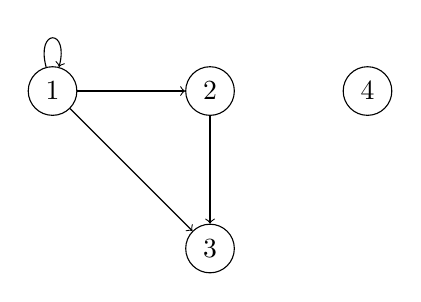
\begin{tikzpicture}[->,node distance=2cm]
  \node[draw,circle] (A) {$1$};
  \node[draw,circle] (B) [right of=A] {$2$};
  \node[draw,circle] (C) [below of=B] {$3$};
  \node[draw,circle] (D) [right of=B] {$4$};
  \draw (A) to [loop above]  (A);
  \draw (A) to  (B);
  \draw (A) to  (C);
  \draw (B) to  (C);
  \end{tikzpicture}
\intertext{This is a different graph than $\tuple{V', E}$ with $V' =
  \{1, 2, 3\}$, which looks like this:}
& 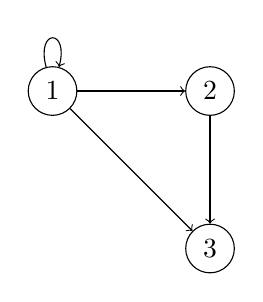
\begin{tikzpicture}[->,node distance=2cm]
  \node[draw,circle] (A) {$1$};
  \node[draw,circle] (B) [right of=A] {$2$};
  \node[draw,circle] (C) [below of=B] {$3$};
  \draw (A) to [loop above]  (A);
  \draw (A) to  (B);
  \draw (A) to  (C);
  \draw (B) to  (C);
  \end{tikzpicture}
\end{align*}
\end{ex}

\begin{prob}
  Consider the less-than-or-equal-to relation~$\le$ on the set $\{1,
  2, 3, 4\}$ as a graph and draw the corresponding diagram.
\end{prob}

\end{document}
